%%%%%%%%%%%%%%%%%%%%%%%%%%%%%%%%%%%%%%
%% Frame
%%%%%%%%%%%%%%%%%%%%%%%%%%%%%%%%%%%%%%

\begin{frame}[t]
	\frametitle{Introduction: Autoencoders}
	\framesubtitle{~~}  %% needed for proper positioning of the logo ...

\begin{figure}[h]
	\centering
	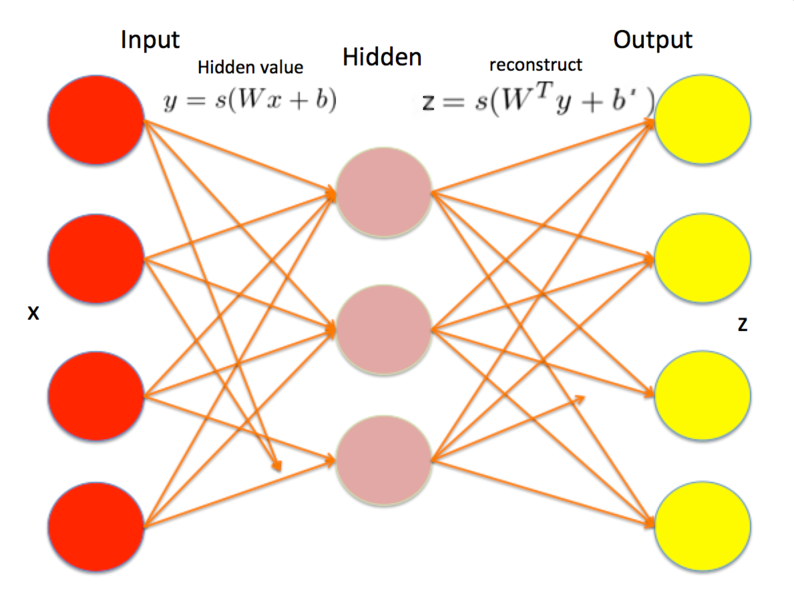
\includegraphics[width=0.7\linewidth]{autoencoder.png}
	\caption{Overview of an autoencoder and its encoding, decoding stages. The weight matrix of the decoding stage is the transpose of the weight matrix of the encoding stage.}
	\label{fig:autoencoder}
\end{figure}


\end{frame}
%%%%%%%%%%%%%%%%%%%%%%%%%%%%%%%%%%%%%
%% Frame
%%%%%%%%%%%%%%%%%%%%%%%%%%%%%%%%%%%%%%
\begin{frame}[t]
	\frametitle{Introduction Autoencoders}
	\framesubtitle{~~}  %% needed for proper positioning of the logo ...

\begin{figure}
  \centering
  \subfloat[]{
    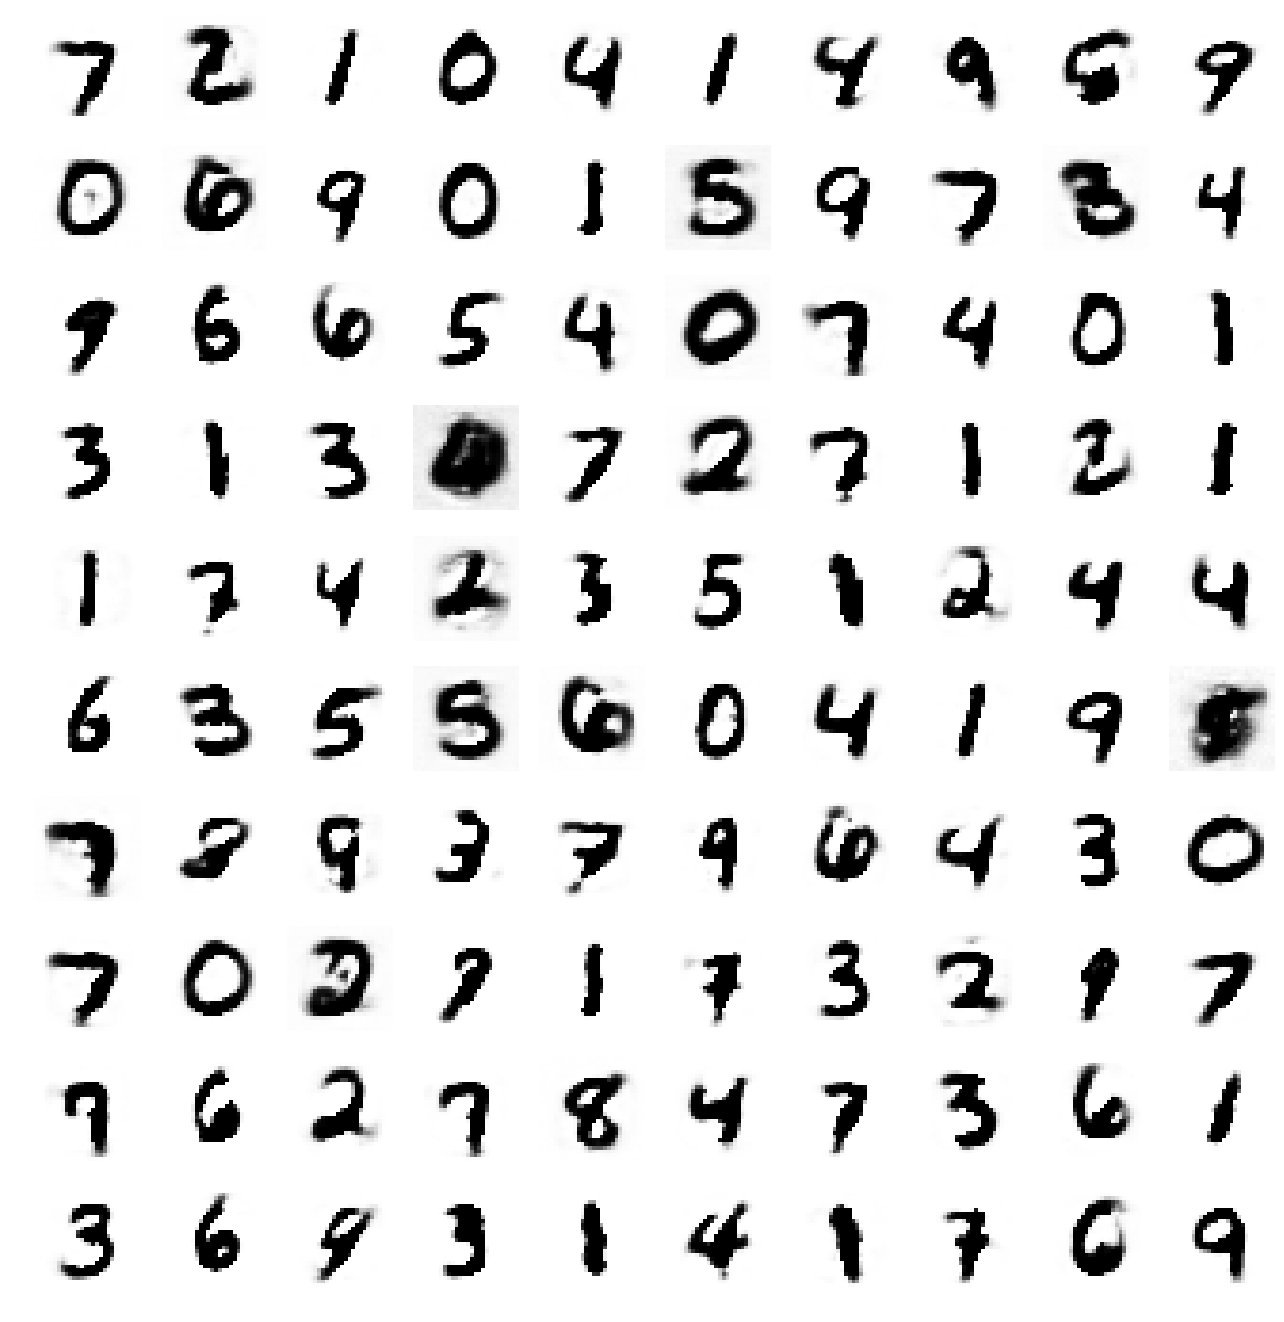
\includegraphics[width=0.4\linewidth]{experiment3_2.png}
  }
  \subfloat[]{
    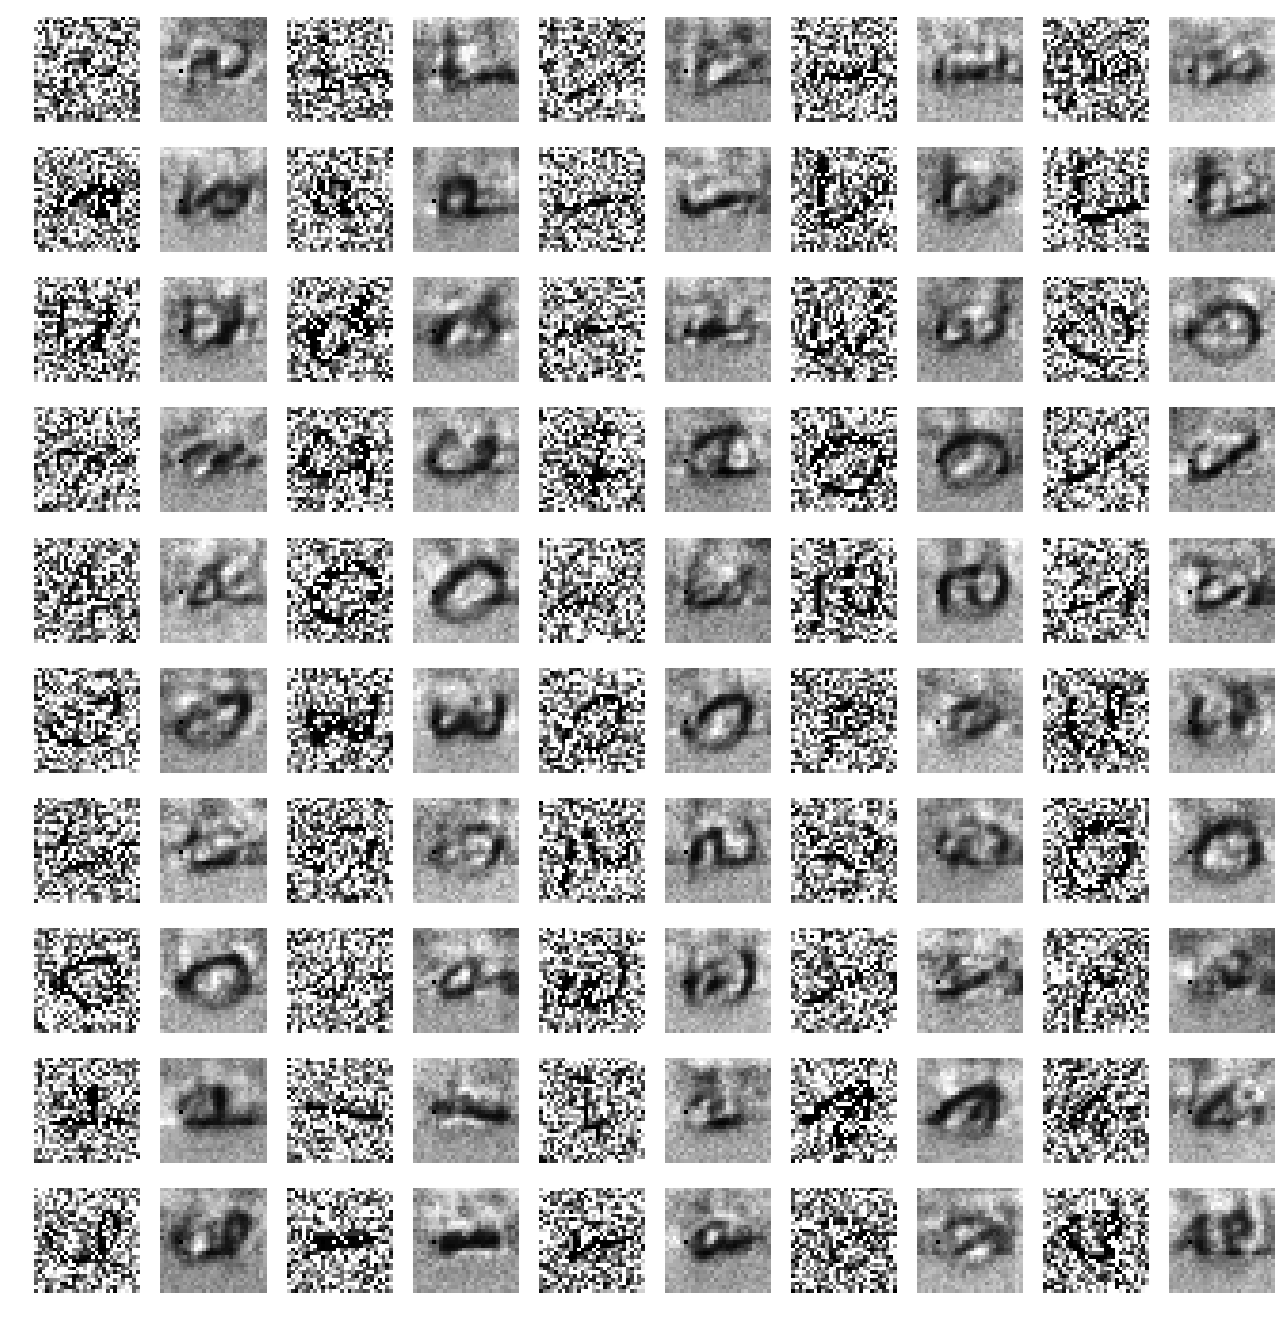
\includegraphics[width=0.4\linewidth]{rand.png}
  }
  \caption{Reconstructions of corrupted digits from the (a) MNIST dataset and  (b) bg-rand dataset}
  \label{fig:reconstruct}
\end{figure}

\end{frame}


%%%%%%%%%%%%%%%%%%%%%%%%%%%%%%%%%%%%%
%% Frame
%%%%%%%%%%%%%%%%%%%%%%%%%%%%%%%%%%%%%%
\begin{frame}[t]
	\frametitle{Introduction Autoencoders}
	\framesubtitle{~~}  %% needed for proper positioning of the logo ...

\begin{figure}
  \centering
  \subfloat[]{
    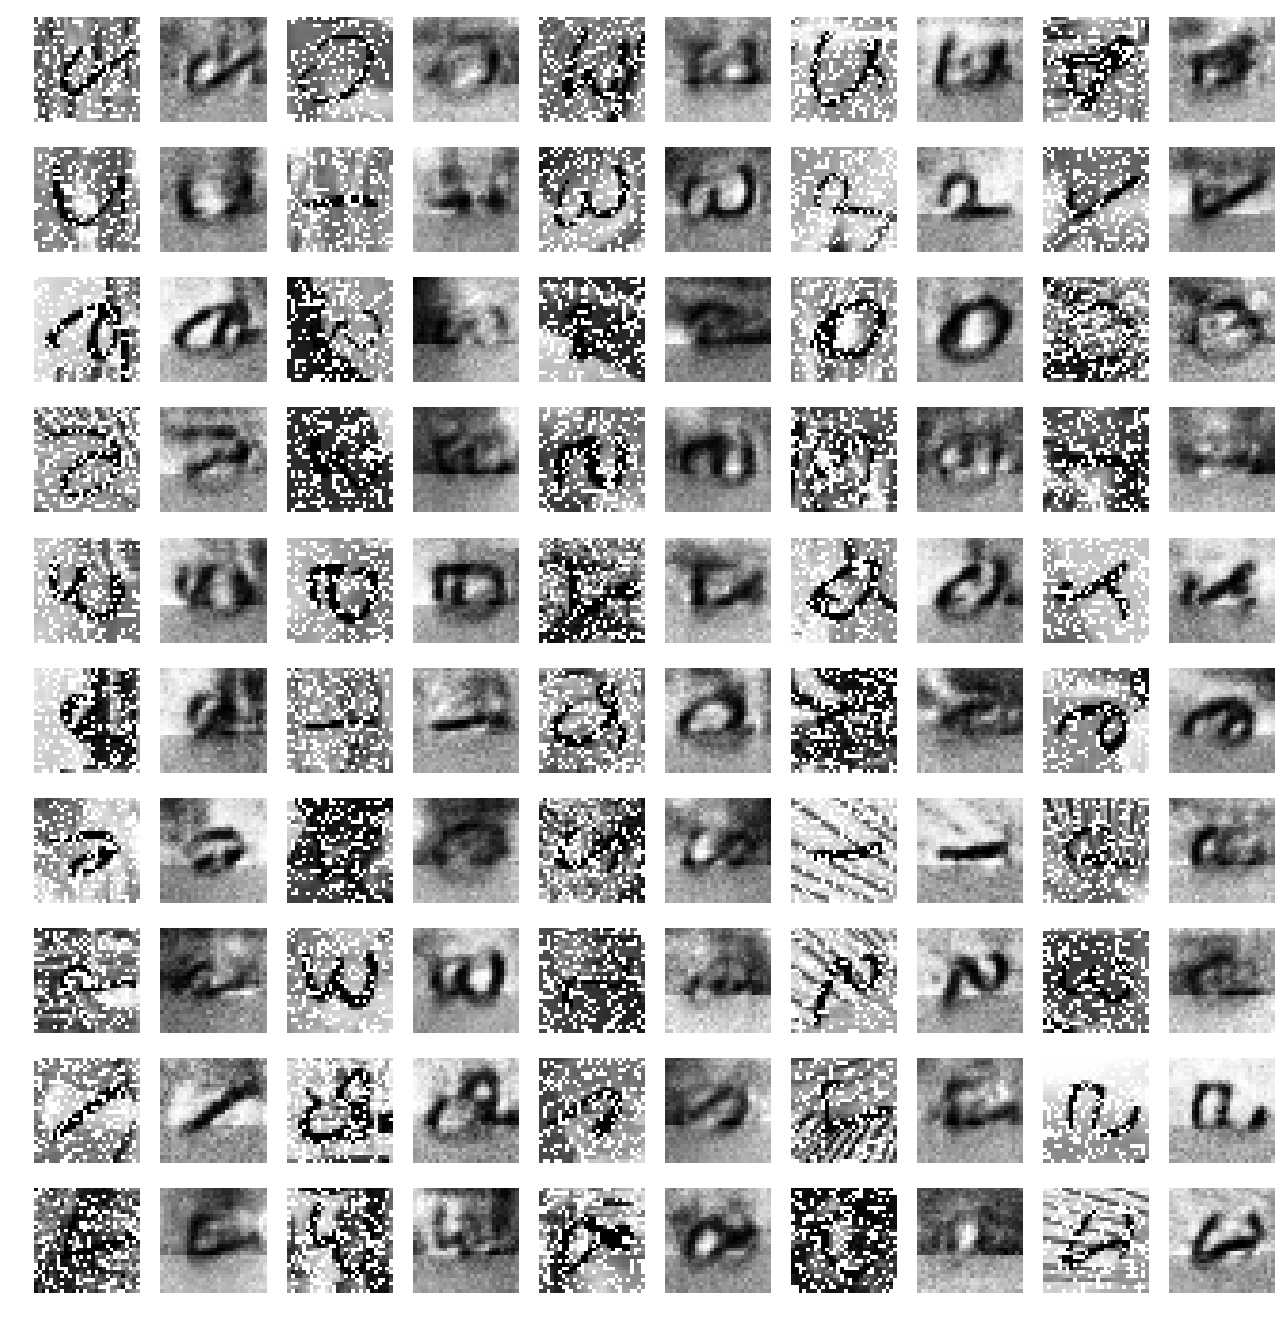
\includegraphics[width=0.4\linewidth]{bg.png}
  }
  \subfloat[]{
    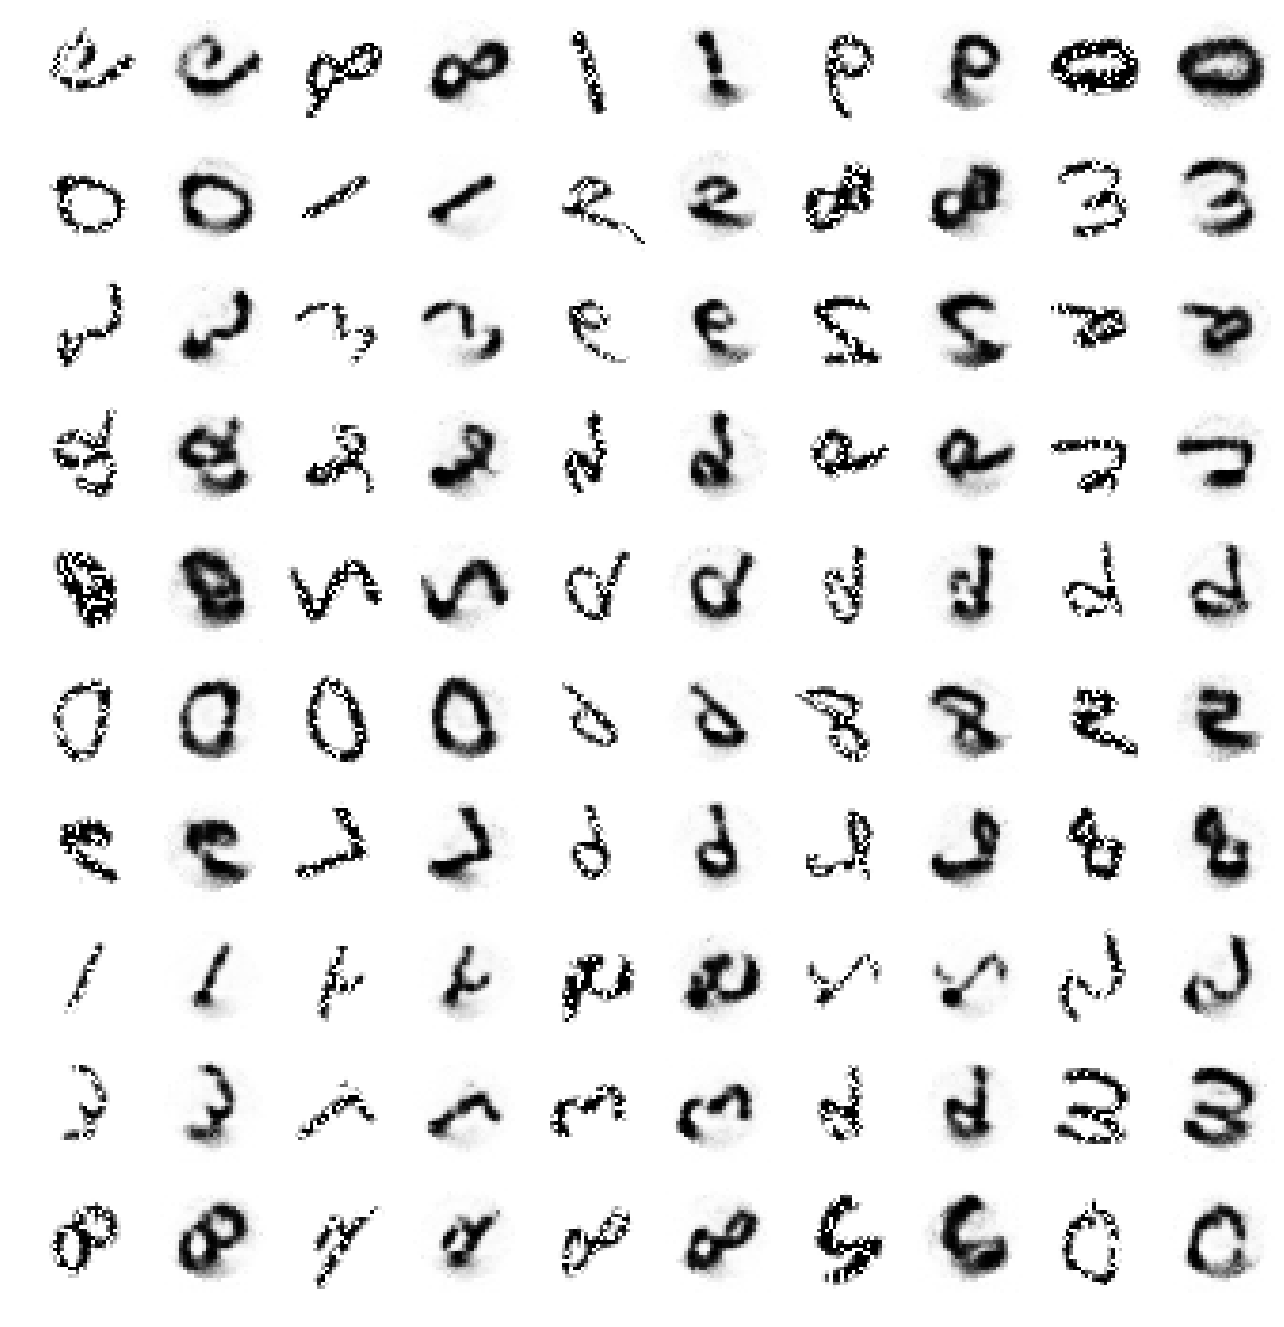
\includegraphics[width=0.4\linewidth]{rot.png}
  }
  \caption{Reconstructions of corrupted digits from the (a) bg-img dataset and (b) rot dataset}
  \label{fig:reconstruct}
\end{figure}

\end{frame}


